\documentclass[lualatex,handout]{beamer}
\setbeamertemplate{footline}[frame number]
\usepackage{luatexja}
\usepackage{amsmath,amssymb}

%\usetheme{Berlin}
\usecolortheme{rose}

\usepackage{tikz}
\usepackage{pgfplots}
\pgfplotsset{compat=1.18}

%\usepackage[haranoaji]{luatexja-preset}
\usepackage[deluxe,ipaex]{luatexja-preset}
\renewcommand{\kanjifamilydefault}{\gtdefault}
%\setmainjfont{HaranoAjiGothic-Regular}

\usepackage{unicode-math}
%\setmathfont{Fira Math}
\setmathfont{STIX Two Math}
\setmathfont{STIX Two Math}[range=bfup/{Latin,latin,num,Greek,greek}]
\setmathfont{STIX Two Math}[range=bfit/{Latin,latin}]
\setmathfont{STIX Two Math}[range={"0000-"FFFF}]
\setmathrm{STIX Two Math}[StylisticSet=8]

%\usefonttheme{professionalfonts}

\usepackage{luacolor}

\newcommand{\mycolor}[2]{%
  \begingroup
  \colorlet{currentcolor}{.}%
  \color{#1}#2%
  \color{currentcolor}%
  \endgroup
}
\newcommand{\emm}[1]{\mycolor{red}{#1}}
\newcommand{\expt}[1]{\mathbb{E}\left[#1\right]}
\newcommand{\var}[1]{\mathbb{V}\left[#1\right]}
\newcommand{\cov}[1]{\mathsf{Cov}\left[#1\right]}
\newcommand{\vc}[1]{\mathsf{Var}\left[#1\right]}


\usepackage{xspace}
%\usepackage{bm}
%\newcommand\bm[1]{{\mathbf{#1}}}
\newcommand\dx{{\,\mathrm{d}x}}

\theoremstyle{definition}

\title{確率・統計基礎: 複数の確率変数、多変量正規分布}
\author{森 立平}
\date{}



\begin{document}
\begin{frame}[plain]
\maketitle
\end{frame}


\begin{frame}{複数の確率変数の確率密度関数}
\footnotesize
%\begin{definition}
\begin{block}{多変数の確率密度関数}
$p_{\symbf{X}}\colon \mathbb{R}^n\to\mathbb{R}$を
$n$次元確率変数$\symbf{X}=[X_1\dotsc X_n]$の\emm{確率密度関数}とすると、
任意の$A\subseteq\mathbb{R}^n$について
%$\stackrel{\mathrm{def}}{\iff}$
\begin{align*}
\Pr(\symbf{X}\in A)&=
%\int_{\substack{-\infty< x_1 \le z_1\\ -\infty< x_2\le z_2\\\vdots\\-\infty<x_n\le z_n}} p_{Z_1,\dotsc,Z_n}(x_1,x_2,\dotsc,x_n)\mathrm{d}{\symbf{x}_1^n}
\int_{A} p_{\symbf{X}}(x)\mathrm{d}x.
\end{align*}
\end{block}
%\end{definition}
%確率変数$Z_1,\dotsc,Z_n$が\emm{独立}のとき、
%\begin{align*}
%p_{Z_1,\dotsc,Z_n}(x_1,\dotsc,x_n)&=p_{Z_1}(x_1)p_{Z_2}(x_2)\dotsm p_{Z_n}(x_n)
%\end{align*}
%である。

\begin{block}{独立な場合}
確率変数$X_1,\dotsc,X_n$が独立な場合、
\begin{align*}
p_{X_1,\dotsc,\, X_n}(x_1,\dotsc, x_n) &= p_{X_1}(x_1)p_{X_2}(x_2)\dotsm p_{X_n}(x_n).
\end{align*}
\end{block}

\begin{example}
$X_1\sim U(0,1)$で($[0,1]$上の一様分布)、$X_2=X_1$のとき$[X_1, X_2]$の確率密度関数は存在しない。
$p_{X_1,\,X_2}(x_1,x_2)$は$x_1\ne x_2$のとき0としてよいが、$p_{X_1,\,X_2}(x,x)$をどのように定義しても$\int_{\mathbb{R}^2}p_{X_1,\,X_2}(x_1,x_2)\mathrm{d}x_1\mathrm{d}x_2=0$になる。
\end{example}

%他の$X_k$の確率密度関数についても同様。
\end{frame}

\begin{frame}{周辺化}
一つの確率変数$X_1$の確率密度関数は
\begin{align*}
\Pr(X_1\in A) &= \Pr(X_1\in A, X_2 \in\mathbb{R},\dotsc, X_n\in\mathbb{R})\\
&=\int_{\substack{x_1\in A\\x_2,\dotsc,x_n\in\mathbb{R}}} p_{X_1,\dotsc,X_n}(x_1,x_2,\dotsc,x_n)\mathrm{d}x\\
&=\int_{x_1\in A}\left(\int_{x_2,\dotsc,x_n\in\mathbb{R}} p_{X_1,\dotsc,X_n}(x_1,x_2,\dotsc,x_n)\mathrm{d}x_2\dotsm \mathrm{d}x_n\right)\mathrm{d}x_1.
%p_{Z_1}(x_1)&=
%%\int_{\substack{-\infty< x_s <\infty \;\forall s\ne 1}} p_{Z_1,\dotsc,Z_n}(x_1,x_2,\dotsc,x_n)\mathrm{d}{\symbf{x}_2^n}.
%\int_{z_2\in\mathbb{R}} p_{Z_1,\dotsc,Z_n}(z_1,z_2,\dotsc,z_n)\mathrm{d}{\symbf{z}_2^n}.
\end{align*}
よって$X_1$の確率密度関数は
\begin{align*}
p_{X_1}(x_1) &=\int_{x_2,\dotsc,x_n\in\mathbb{R}} p_{X_1,\dotsc,X_n}(x_1,x_2,\dotsc,x_n)\mathrm{d}x_2\dotsm \mathrm{d}x_n
\end{align*}
\end{frame}

\begin{frame}{期待値}
確率変数のベクトルや行列に対する$\expt{\cdot}$は成分毎に期待値を取ることを表す。
\begin{align*}
\symbf{X} &= \begin{bmatrix}X_1\\X_2\\\vdots\\X_n\end{bmatrix}&\text{とすると}\qquad
\expt{\symbf{X}} &= \begin{bmatrix}\expt{X_1}\\\expt{X_2}\\\vdots\\\expt{X_n}\end{bmatrix}
\end{align*}
である。
\end{frame}

\begin{frame}{分散共分散行列}
\small
\begin{definition}[分散共分散行列]
確率変数$X_1,\dotsc,X_n$の\emm{分散共分散行列}(もしくは\emm{共分散行列})$\vc{\symbf{X}}\in\mathbb{R}^{n\times n}$は
$(i,\,j)$成分に$\cov{X_i,\,X_j}=\expt{X_iX_j}-\expt{X_i}\expt{X_j}$を持つ行列である。
\end{definition}
\begin{align*}
\vc{\symbf{X}}&=
\begin{bmatrix}
\var{X_1}&\cov{X_1,X_2}&\cov{X_1,X_3}\\
\cov{X_2,X_1}&\var{X_2}&\cov{X_2,X_3}\\
\cov{X_3,X_1}&\cov{X_3,X_2}&\var{X_3}\\
\end{bmatrix}
\end{align*}
分散共分散行列は以下のように表せる。
\begin{align*}
\vc{\symbf{X}}&=
\expt{\symbf{X} \symbf{X}^T} - \expt{\symbf{X}}\expt{\symbf{X}}^T
\end{align*}
\end{frame}

\begin{frame}{分散共分散行列の性質}
\begin{itemize}
\setlength{\itemsep}{2em}
\item $\vc{\symbf{X}}$は対称行列である。
\item $\vc{\symbf{X}}$は半正定値である。
\item $\vc{\symbf{X}+b}=\vc{\symbf{X}}\quad\forall b\in\mathbb{R}^n$.
\item $\vc{A\symbf{X}}=A\vc{\symbf{X}}A^T\quad\forall A\in\mathbb{R}^{m\times n}$.
%\item $\vc{\symbf{X}+\symbf{Y}}=\vc{\symbf{X}} + \vc{\symbf{Y}} + $.
\end{itemize}
\end{frame}

\begin{frame}{線形変換の分散共分散行列}
行列$A\in\mathbb{R}^{m\times n}$と$n\times k$の確率変数行列$\symbf{R}$について$\expt{A\symbf{R}}=A\expt{\symbf{R}}$である。
よって、$N$次元確率変数ベクトル$\symbf{X}$について
\begin{align*}
&\emm{\expt{(\symbf{X} - \expt{\symbf{X}})(\symbf{X} - \expt{\symbf{X}})^T}}\\
=&\expt{\symbf{X}\symbf{X}^T - \symbf{X}\expt{\symbf{X}}^T - \expt{\symbf{X}}\symbf{X}^T + \expt{\symbf{X}}\expt{\symbf{X}}^T}\\
=& \expt{\symbf{X} \symbf{X}^T} - \expt{\symbf{X}}\expt{\symbf{X}}^T
=\vc{\symbf{X}}
\end{align*}
よって$\vc{\symbf{X}+b}=\vc{\symbf{X}}$である。

\vspace{1em}
\begin{align*}
\vc{A\symbf{X}}&=\expt{A\symbf{X} (A\symbf{X})^T} - \expt{A\symbf{X}}\expt{A\symbf{X}}^T\\
&=A\expt{\symbf{X} \symbf{X}^T}A^T - A\expt{\symbf{X}}\expt{\symbf{X}}^TA^T\\
&=A\emm{\vc{\symbf{X}}}A^T
\end{align*}
\end{frame}

\begin{frame}{分散共分散行列の半正定値性 I}
\small
\begin{align*}
&
\begin{bmatrix}
1&\expt{X_1}&\expt{X_2}&\expt{X_3}\\
\expt{X_1}&\expt{X_1^2}&\expt{X_1X_2}&\expt{X_1X_3}\\
\expt{X_2}&\expt{X_2X_1}&\expt{X_2^2}&\expt{X_2X_3}\\
\expt{X_3}&\expt{X_3X_1}&\expt{X_3X_2}&\expt{X_3^2}\\
\end{bmatrix}\\
=&
\expt{
\begin{bmatrix}
1&X_1&X_2&X_3\\
X_1&X_1^2&X_1X_2&X_1X_3\\
X_2&X_2X_1&X_2^2&X_2X_3\\
X_3&X_3X_1&X_3X_2&X_3^2\\
\end{bmatrix}}\\
=&
\expt{
\begin{bmatrix}
1\\
X_1\\
X_2\\
X_3\\
\end{bmatrix}
\begin{bmatrix}
1&
X_1&
X_2&
X_3
\end{bmatrix}}\ge 0\qquad (\text{\emm{半正定値行列の期待値は半正定値}})
\end{align*}

任意の$a\in\mathbb{R}^n$ と$n\times n$半正定値ランダム行列$R$について
$a^T \expt{R}a = \expt{a^TR a}\ge 0$
なので$\expt{R}\ge0$.
\end{frame}

\begin{frame}{分散共分散行列の半正定値性 II}
\scriptsize
\begin{align*}
&
\begin{bmatrix}
-\expt{X_1}&1&0&0\\
-\expt{X_2}&0&1&0\\
-\expt{X_3}&0&0&1\\
\end{bmatrix}
\begin{bmatrix}
1&\expt{X_1}&\expt{X_2}&\expt{X_3}\\
\expt{X_1}&\expt{X_1^2}&\expt{X_1X_2}&\expt{X_1X_3}\\
\expt{X_2}&\expt{X_2X_1}&\expt{X_2^2}&\expt{X_2X_3}\\
\expt{X_3}&\expt{X_3X_1}&\expt{X_3X_2}&\expt{X_3^2}\\
\end{bmatrix}\\
=&
\begin{bmatrix}
0&\expt{X_1^2}-\expt{X_1}^2&\expt{X_1X_2}-\expt{X_1}\expt{X_2}&\expt{X_1X_3}-\expt{X_1}\expt{X_3}\\
0&\expt{X_2X_1}-\expt{X_2}\expt{X_1}&\expt{X_2^2}-\expt{X_2}^2&\expt{X_2X_3}-\expt{X_2}\expt{X_3}\\
0&\expt{X_3X_1}-\expt{X_3}\expt{X_1}&\expt{X_3X_2}-\expt{X_3}\expt{X_2}&\expt{X_3^2}-\expt{X_3}^2\\
\end{bmatrix}\\
\end{align*}
\begin{align*}
&
\begin{bmatrix}
0&\var{X_1}&\cov{X_1, X_2}&\cov{X_1, X_3}\\
0&\cov{X_2, X_1}&\var{X_2}&\cov{X_2, X_3}\\
0&\cov{X_3, X_1}&\cov{X_3, X_2}&\var{X_3}
\end{bmatrix}
\begin{bmatrix}
-\expt{X_1}& -\expt{X_2}& -\expt{X_3}\\
1&0&0\\
0&1&0\\
0&0&1\\
\end{bmatrix}\\
&=\vc{\symbf{X}}
\end{align*}

$A\ge 0$のとき任意の行列$B$について$BAB^T\ge 0$なので$\vc{\symbf{X}}\ge 0$である。
\end{frame}

\begin{frame}{多変量正規分布}
\begin{definition}[多変量正規分布]
平均$\mu\in\mathbb{R}^n$、分散共分散行列$\Sigma\in\mathbb{R}^{n\times n}_{>0}$の
多変量正規分布$N(\mu,\,\Sigma)$に従う $n$次元確率変数$\symbf{Z}$の確率密度関数は
\begin{align*}
p_{\symbf{Z}}(x) &= \frac1{\sqrt{(2\pi)^n\det(\Sigma)}} \mathrm{e}^{-\frac12 (x-\symbf{\mu})^T\Sigma^{-1} (x-\symbf{\mu})}
\qquad \text{for }x\in\mathbb{R}^n
\end{align*}
で定義される。

また、$n\times n$単位行列$I_n$について$N(0,\, I_n)$は\emm{$n$次元標準正規分布}と呼ばれる。
\end{definition}
\end{frame}
\begin{frame}{確率密度関数}
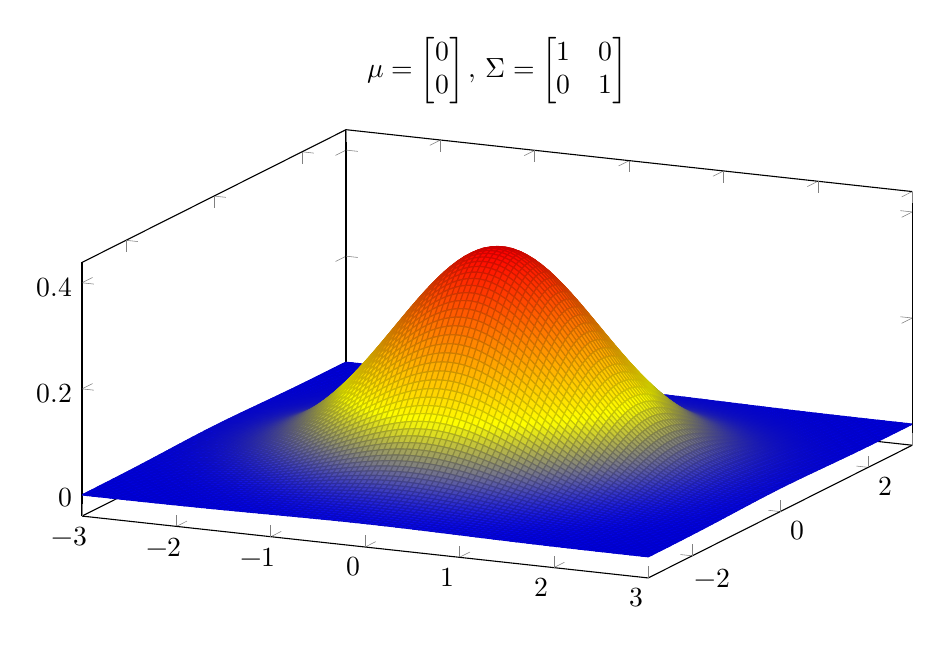
\begin{tikzpicture}
\begin{axis}[
%    title={$\frac1{2\pi}\mathrm{e}^{-\frac12(x^2+y^2)}$},
    title={$\mu=\begin{bmatrix}0\\0\end{bmatrix},\,\Sigma = \begin{bmatrix}1&0\\0&1\end{bmatrix}$},
    width=\textwidth, height=\axisdefaultheight,
%%    zlabel={$p(x,y)$},
%    xlabel={$x$},
%    ylabel={$y$},
%    xmin=-3, xmax=3,
%    ymin=-3, ymax=3,
%    scaled ticks = false,
%    isosamples=100,
%    pm3d = true
    %tick label style={/pgf/number format/assume math mode=true, font=\footnotesize\sffamily},
    %yticklabel style={/pgf/number format/.cd, fixed, fixed zerofill, precision=2},
    %    domain=0:\binomN,samples at={0,1,...,\binomN},
    %mark options={scale=0.75, blue},
    %ybar, bar width = .75pt
        ]
%\addplot[ycomb] {binom(x,\binomN,0.3)};
%\addplot {binom(x,\binomN,0.3)};
\addplot3[surf, domain=-3:3, samples=100] {1.0/sqrt(2*pi) * exp(-0.5*(x^2 + y^2))};
\end{axis}
\end{tikzpicture}
\end{frame}

\begin{frame}{確率密度関数}
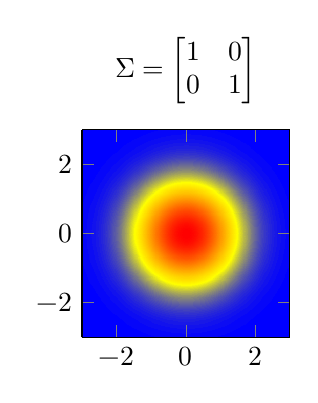
\begin{tikzpicture}
\begin{axis}[
    title={$\Sigma = \begin{bmatrix}1&0\\0&1\end{bmatrix}$},
    width=120, height=120,
    view={0}{90},
    %colorbar horizontal
        ]
\addplot3[contour filled={number=128}, domain=-3:3, samples=100] {1.0/sqrt(2*pi) * exp(-0.5*(x^2 + y^2))};
\end{axis}
\end{tikzpicture}
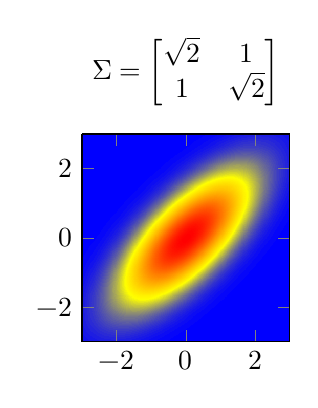
\begin{tikzpicture}
\begin{axis}[
    title={$\Sigma = \begin{bmatrix}\sqrt{2}&1\\1&\sqrt{2}\end{bmatrix}$},
    width=120, height=120,
    view={0}{90},
    %colorbar horizontal
        ]
\addplot3[contour filled={number=128}, domain=-3:3, samples=100] {1.0/sqrt(2*pi) * exp(-0.5*(sqrt(2)*x^2 + sqrt(2)*y^2 - 2*x*y))};
\end{axis}
\end{tikzpicture}
%
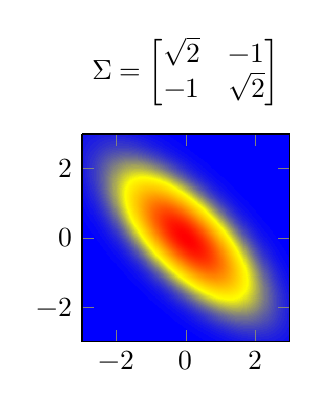
\begin{tikzpicture}
\begin{axis}[
    title={$\Sigma = \begin{bmatrix}\sqrt{2}&-1\\-1&\sqrt{2}\end{bmatrix}$},
    width=120, height=120,
    view={0}{90},
    %colorbar horizontal
        ]
\addplot3[contour filled={number=128}, domain=-3:3, samples=100] {1.0/sqrt(2*pi) * exp(-0.5*(sqrt(2)*x^2 + sqrt(2)*y^2 + 2*x*y))};
\end{axis}
\end{tikzpicture}
\end{frame}

\begin{frame}{密度関数の積分}
\small
多変量正規分布の密度関数を積分して1になることを確認する。
$\Sigma$は対称行列なのである\emm{直交行列$V$}と\emm{対角行列$D$}が存在して\emm{$\Sigma=V^TDV$}と表せる(スペクトル分解)。
また$\Sigma$は正定値なので、$D$の対角成分は正である。
\begin{align*}
&\int_{\mathbb{R}^n} \frac1{\sqrt{(2\pi)^n\det(\Sigma)}} \mathrm{e}^{-\frac12 (x-\symbf{\mu})^T\Sigma^{-1} (x-\symbf{\mu})}\mathrm{d}x\\
&=
\int_{\mathbb{R}^n} \frac1{\sqrt{(2\pi)^n\det(\Sigma)}} \mathrm{e}^{-\frac12 x^T\Sigma^{-1} x}\mathrm{d}x\\
&=
\int_{\mathbb{R}^n} \frac1{\sqrt{(2\pi)^n\det(D)}} \mathrm{e}^{-\frac12 (Vx)^TD^{-1} (Vx)}\mathrm{d}x\qquad(\Sigma=V^TDV)\\
&=
\int_{\mathbb{R}^n} \frac1{\sqrt{(2\pi)^n\det(D)}} \mathrm{e}^{-\frac12 y^TD^{-1} y}\frac1{|\det(V)|}\mathrm{d}y\qquad (y=Vx)\\
&=
\int_{\mathbb{R}^n} \frac1{\sqrt{(2\pi)^n\det(D)}} \mathrm{e}^{-\frac12 z^T z}\frac1{\left|\det(\sqrt{D^{-1}})\right|}\mathrm{d}z\qquad (z=\sqrt{D^{-1}}y)\\
&=
\int_{\mathbb{R}^n} \frac1{\sqrt{(2\pi)^n}} \mathrm{e}^{-\frac12 z^T z}\mathrm{d}z
=\prod_{k=1}^n\left(\int_{-\infty}^\infty \frac1{\sqrt{2\pi}}\mathrm{e}^{-\frac{z_k^2}2}\mathrm{d}z_k\right) = 1
\end{align*}
\end{frame}

\begin{frame}{多変数のモーメント母関数、キュムラント母関数、特性関数}
\small
\begin{definition}[多変数モーメント母関数]
$n$次元確率変数${\symbf{X}}$の\emm{モーメント母関数}$\varphi_{{\symbf{X}}}\colon\mathbb{R}^n\to\mathbb{R}$を以下で定義する。
\begin{align*}
M_{{\symbf{X}}}(t) &:= \expt{\mathrm{e}^{\langle t,\, {\symbf{X}}\rangle}}.
\end{align*}
ここで$\langle t,\, {\symbf{X}}\rangle := \emm{\sum_{k=1}^n t_k X_k}$である。

また\emm{キュムラント母関数}を$K_{\symbf{X}}(t) := \log M_{\symbf{X}}(t)$と定義する。
\end{definition}
\begin{definition}[多変数特性関数]
$n$次元確率変数${\symbf{X}}$の\emm{特性関数}$\varphi_{{\symbf{X}}}\colon\mathbb{R}^n\to\mathbb{C}$を以下で定義する。
\begin{align*}
\varphi_{{\symbf{X}}}(t) &:= \expt{\mathrm{e}^{i\langle t,\, {\symbf{X}}\rangle}}.
\end{align*}
%ここで$\langle t,\, X\rangle := \sum_{k=1}^n t_k X_k$である。
\end{definition}
\end{frame}

\begin{frame}{多変数のモーメント母関数、キュムラント母関数、特性関数の性質}
\small
\begin{itemize}
\setlength{\itemsep}{1em}
\item $M_{\symbf{X}}(t)$が原点を含む開集合で存在するとき、この範囲で無限回微分できる(ルベーグ積分に基づいた議論が必要)。
このとき、$t$に関する微分と期待値の順番を交換できる。
\begin{align*}
%\left.\frac{\mathrm{d}^k\varphi_X(t)}{\mathrm{d}t^k}\right|_{t=0} &= i^k \expt{X^k}.
\left.\frac{\partial M_{\symbf{X}}(t)}{\partial t_k}\right|_{t=0} &= \left.\expt{X_k\mathrm{e}^{\langle t,\, {\symbf{X}}\rangle}}\right|_{t=0} = \expt{X_k}\\
\left.\frac{\partial^2 M_{\symbf{X}}(t)}{\partial t_k\partial t_\ell}\right|_{t=0} &= \left.\expt{X_kX_\ell\mathrm{e}^{\langle t,\, {\symbf{X}}\rangle}}\right|_{t=0} = \expt{X_kX_\ell}\\
\left.\frac{\partial K_{\symbf{X}}(t)}{\partial t_k}\right|_{t=0} &= \left.\frac{\expt{X_k\mathrm{e}^{\langle t,\, {\symbf{X}}\rangle}}}{\expt{\mathrm{e}^{\langle t,\, {\symbf{X}}\rangle}}}\right|_{t=0} = \expt{X_k}\\
\left.\frac{\partial^2 K_{\symbf{X}}(t)}{\partial t_k\partial t_\ell}\right|_{t=0} &= \left.\frac{\expt{X_kX_\ell\mathrm{e}^{\langle t,\, {\symbf{X}}\rangle}}}{\expt{\mathrm{e}^{\langle t,\, {\symbf{X}}\rangle}}}\right|_{t=0} - \left(\left.\frac{\expt{X_k\mathrm{e}^{\langle t,\, {\symbf{X}}\rangle}}}{\expt{\mathrm{e}^{\langle t,\, {\symbf{X}}\rangle}}}\right|_{t=0}\right)\left(\left.\frac{\expt{X_\ell\mathrm{e}^{\langle t,\, {\symbf{X}}\rangle}}}{\expt{\mathrm{e}^{\langle t,\, {\symbf{X}}\rangle}}}\right|_{t=0}\right)\\
&= \expt{X_kX_\ell} - \expt{X_k}\expt{X_\ell} = \cov{X_k, X_\ell}.
\end{align*}
\item ${\symbf{X}}$と$\symbf{Y}$の分布が同じ$\emm{\iff}\varphi_{\symbf{X}}=\varphi_{\symbf{Y}}$ (ルベーグ積分に基づいた議論が必要)。
\end{itemize}


\vspace{1em}
%$X$が$k$次モーメントを持つ$\iff$$\varphi_X$は0で$k$回微分できる。
\end{frame}

\begin{frame}{多変数のモーメント母関数の性質}
\small
\begin{itemize}
\setlength{\itemsep}{3em}
\item 任意の$n$次元確率変数$\symbf{X}$と$b\in\mathbb{R}^n$について
$M_{{\symbf{X}}\emm{+b}}(t) = \expt{\mathrm{e}^{\langle t,\, {\symbf{X}}+b\rangle}} = \expt{\mathrm{e}^{\langle t,\,\symbf{X}\rangle}\mathrm{e}^{\langle t,\,b\rangle}} = \expt{\mathrm{e}^{\langle t,\, {\symbf{X}}\rangle}}\mathrm{e}^{\langle t,\,b\rangle}$\\
$\qquad = M_{\symbf{X}}(t)\emm{\mathrm{e}^{\langle t,\, b\rangle}}$.
\item 任意の$n$次元確率変数$\symbf{X}$と$A\in\mathbb{R}^{m\times n}$について
$M_{\emm{A}{\symbf{X}}}(t) = \expt{\mathrm{e}^{\langle t,\, A{\symbf{X}}\rangle}} = \expt{\mathrm{e}^{\langle A^Tt,\, {\symbf{X}}\rangle}} = M_{\symbf{X}}(\emm{A^T}t)$.
\item 任意の独立$n$次元確率変数$\symbf{X}$と$\symbf{Y}$について
$M_{{\symbf{X}}\emm{+}{\symbf{Y}}}(t) = \expt{\mathrm{e}^{\langle t,\, {\symbf{X}}+{\symbf{Y}}\rangle}} = \expt{\mathrm{e}^{\langle t,\, {\symbf{X}}\rangle}}\expt{\mathrm{e}^{\langle t,\, {\symbf{Y}}\rangle}}= \emm{M_{\symbf{X}}(t)M_{\symbf{Y}}(t)}$.
\end{itemize}
\end{frame}

\begin{frame}{多変量正規分布のキュムラント母関数}
\small
\begin{align*}
&\expt{\mathrm{e}^{\langle t,\,\symbf{Z}\rangle}}\\
&=\int_{-\infty}^\infty \frac1{\sqrt{(2\pi)^n\det(\Sigma)}} \mathrm{e}^{-\frac12 (x-\mu)^T\Sigma^{-1} (x-\mu)}\mathrm{e}^{\langle t,\, x\rangle}\mathrm{d}x\\
&= \int_{-\infty}^\infty \frac1{\sqrt{(2\pi)^n\det(\Sigma)}} \mathrm{e}^{-\frac12 \left\langle\Sigma^{-\frac12}(x-\mu),\,\Sigma^{-\frac12}(x-\mu)\right\rangle+\left\langle \Sigma^{\frac12}t,\, \Sigma^{-\frac12}x\right\rangle}\mathrm{d}x\\
&= \int_{-\infty}^\infty \frac1{\sqrt{(2\pi)^n\det(\Sigma)}} \mathrm{e}^{-\frac12 \left\langle\Sigma^{-\frac12}(x-\mu-\Sigma t),\,\Sigma^{-\frac12}(x-\mu-\Sigma t)\right\rangle +\left\langle \mu,\, t\right\rangle + \frac12\left\langle \Sigma^\frac12t,\,\Sigma^\frac12t\right\rangle}\mathrm{d}x\\
&= \mathrm{e}^{\langle \mu,\, t\rangle + \frac12\langle \Sigma^\frac12t,\,\Sigma^\frac12t\rangle}.
\end{align*}
よって、$K_{\symbf{Z}}(t) = \emm{\langle \mu,\, t\rangle + \frac12\left\langle \Sigma^\frac12t,\,\Sigma^\frac12t\right\rangle}$.
\begin{align*}
\left.\frac{\partial K_{\symbf{Z}}(t)}{\partial t_k}\right|_{t=0} &= \mu_k\\
\left.\frac{\partial^2 K_{\symbf{Z}}(t)}{\partial t_k\partial t_\ell}\right|_{t=0} &= \Sigma_{k, \ell}.
\end{align*}
\end{frame}

\begin{frame}{多変量正規分布の周辺化も多変量正規分布}
\begin{lemma}
$n$次元の確率変数$\symbf{Z}=[Z_1,\dotsc, Z_n]\sim N(\mu, \Sigma)$について、
$\symbf{Z}':=[Z_1,\dotsc, Z_{n-1}]\sim N(\mu', \Sigma')$.
ここで、$\mu'\in\mathbb{R}^{N-1}$は$\mu$の第$n$成分を除いたもので$\Sigma'$は$\Sigma$の$n$行目と$n$列目を除いたもの。
\end{lemma}
\begin{proof}
\begin{align*}
\varphi_{\symbf{Z}'}(t') &= \expt{\mathrm{e}^{i\langle t',\,\symbf{Z}'\rangle}}\\
&=\expt{\mathrm{e}^{i\langle t',\, \symbf{Z}'\rangle + 0\cdot Z_n}}\\
&=\varphi_{\symbf{Z}}(t',0) = \mathrm{e}^{i\langle t',\,\mu'\rangle - \langle \sqrt{\Sigma'}t',\,\sqrt{\Sigma'}t'\rangle}.
\end{align*}
\end{proof}
\end{frame}

\begin{frame}{多変量正規分布の一次変換}
\small
\begin{lemma}
$n$次元の確率変数$\symbf{Z}\sim N(\mu, \Sigma)$とランク$m$行列$A\in\mathbb{R}^{m\times n}$と$b\in\mathbb{R}^m$について、
$A\symbf{Z}+b\sim N(\emm{A\mu+b}, \emm{A\Sigma A^T})$.
%$Z_k\sim N(\mu_k, \Sigma_{k,k})$.
\end{lemma}
\begin{proof}
$\varphi_{\symbf{Z}}(t) = \mathrm{e}^{i\langle \mu,\, t\rangle - \frac12\langle \Sigma^\frac12t,\,\Sigma^\frac12t\rangle}$より、
\begin{align*}
\varphi_{A{\symbf{Z}}+b}(t) &= \varphi_{A{\symbf{Z}}}(t)\mathrm{e}^{i\langle t,\,b\rangle} = \varphi_{\symbf{Z}}(A^Tt)\mathrm{e}^{i\langle t,\,b\rangle}\\
&= \mathrm{e}^{i\langle \mu,\, A^T t\rangle - \frac12\langle \Sigma^\frac12A^T t,\,\Sigma^\frac12A^T t\rangle + i\langle t,\,b\rangle}\\
&= \mathrm{e}^{i\langle A\mu,\, t\rangle - \frac12\langle \Sigma^\frac12A^T t,\,\Sigma^\frac12A^T t\rangle+ i\langle t,\,b\rangle}\\
&= \mathrm{e}^{i\langle A\mu + b,\, t\rangle - \frac12\langle \Sigma^\frac12A^T t,\,\Sigma^\frac12A^T t\rangle}\\
&= \mathrm{e}^{i\langle A\mu + b,\, t\rangle - \frac12\langle t,\,A \Sigma A^T t\rangle}.
\end{align*}
これは$N(A\mu+b,\, A\Sigma A^T)$の特性関数である。
\end{proof}
\end{frame}

\begin{frame}{逆関数法: 一様分布から一般の分布の作り方}
\footnotesize
\begin{theorem}[逆関数法]
$U\sim U(0,1)$とすると、任意の確率変数$X$と\emm{$F^{-1}_X(U)$}は同じ分布を持つ。
ここで、$F_X$は$X$の累積分布関数であり
\begin{align*}
F_X^{-1}(p) &:= \inf\left\{ x\in\mathbb{R}\mid F_X(x)\ge p\right\} \qquad\forall p\in[0,1].
\end{align*}
\end{theorem}
\begin{proof}

\vspace{-2em}
\begin{align*}
\Pr(F_X^{-1}(U)\le x) &=
%\Pr(F_X(F_X^{-1}(U))\le F_X(x))\\
%&=
\Pr(U\le F_X(x))
=F_X(x)
\end{align*}
最初の等号は以下の関係から従う。
\begin{align*}
F_X^{-1}(u)\le x &\iff u\le F_X(x)
\end{align*}
$\implies:$ $F_X$が右連続であることに注意すると$u\le F_X(F_X^{-1}(u))$なので
\begin{align*}
F_X^{-1}(u)\le x &\implies F_X(F^{-1}_X(u))\le F_X(x).
 \implies u\le F_X(x)
\end{align*}
$\impliedby:$ $F_X^{-1}(F_X(x))\le x$より
\begin{align*}
u\le F_X(x) &\implies F_X^{-1}(u)\le F_X^{-1}(F_X(x)) \implies F_X^{-1}(u)\le x.
\end{align*}
\end{proof}
\end{frame}

\if0
\begin{frame}{$\chi$二乗分布}
$k$個の独立確率変数が$X_1,\dotsc,X_k\sim N(0,1)$のとき
\begin{align*}
\sum_{s=1}^k X_s^2
\end{align*}
が従う分布を\emm{自由度$k$の$\chi$二乗分布}といい$\chi_k^2$と表す。
\end{frame}

%\begin{frame}{標準正規分布に従う確率変数の二乗}
\begin{frame}{自由度1の$\chi$二乗分布}
\small
$f(x)=x^2$は単調関数ではないが$Z$の確率密度関数が対称($p(-z)=p(z)$)のとき、
\begin{align*}
\Pr(Z^2\le x) &= \Pr(Z\in [-\sqrt{x},\,\sqrt{x}])\\
&= \int_{-\sqrt{x}}^{\sqrt{x}} p(z)\mathrm{d}z\\
&= \int_{0}^{\sqrt{x}} p(z)\mathrm{d}z + \int_{-\sqrt{x}}^{0} p(z)\mathrm{d}z\\
&= 2\int_{0}^{\sqrt{x}} p(z)\mathrm{d}z \qquad (p(-z)=p(z))\\
&= 2\int_{0}^{x} p(\sqrt{u})\frac1{2\sqrt{u}}\mathrm{d}u \qquad (u = z^2)
\end{align*}

ここで$Z\sim N(0,1)$のとき、$Z^2$の確率密度関数は以下になる。
\begin{align*}
\emm{\frac1{\sqrt{2\pi x}} \mathrm{e}^{-\frac12 x}}\qquad x \ge 0.
\end{align*}
\end{frame}


\begin{frame}{ガウス積分}
\begin{align*}
&\left(\int_{-\infty}^\infty \frac1{\sqrt{2\pi}}\mathrm{e}^{-\frac12x^2}\mathrm{d}x\right)^2
=
\left(\int_{-\infty}^\infty \frac1{\sqrt{2\pi}}\mathrm{e}^{-\frac12x^2}\mathrm{d}x\right)
\left(\int_{-\infty}^\infty \frac1{\sqrt{2\pi}}\mathrm{e}^{-\frac12y^2}\mathrm{d}y\right)\\
&=
\int_{\mathbb{R}^2} \frac1{2\pi}\mathrm{e}^{-\frac12(x^2+y^2)}\mathrm{d}x\mathrm{d}y\\
&=
\int_{0\le r,\, \theta\in[0,2\pi)} \frac1{2\pi}\mathrm{e}^{-\frac12r^2}r\mathrm{d}r\mathrm{d}\theta\qquad \left(r = \det\left(\begin{bmatrix}\cos\theta&\sin\theta\\-r\sin\theta&r\cos\theta\end{bmatrix}\right)\right)\\
&=
\emm{
\left(\int_{0}^\infty r\mathrm{e}^{-\frac12r^2}\mathrm{d}r\right)
\left(\int_0^{2\pi} \frac1{2\pi}\mathrm{d}\theta\right)}\\
&=\left[-\mathrm{e}^{-\frac12r^2}\right]_0^\infty\cdot 1 = 1
\end{align*}
\end{frame}

\begin{frame}{自由度2の$\chi$二乗分布}
$Z$を自由度2の$\chi$二乗分布に従う確率変数とすると、任意の$A\subseteq\mathbb{R}^2$について
\begin{align*}
\Pr(Z\le z) &= \Pr(X^2 + Y^2 \le z)\\
&= \int_{x^2+y^2\le z} \frac1{2\pi}\mathrm{e}^{-\frac12(x^2+y^2)}\mathrm{d}x\mathrm{d}y\\
&=
\int_{0\le r\le \sqrt{z},\, \theta\in[0,2\pi)} \frac1{2\pi}\mathrm{e}^{-\frac12r^2}r\mathrm{d}r\mathrm{d}\theta\\
&=
\left(\int_{0}^{\sqrt{z}} r\mathrm{e}^{-\frac12r^2}\mathrm{d}r\right)
\left(\int_0^{2\pi} \frac1{2\pi}\mathrm{d}\theta\right)\\
&=\left[-\mathrm{e}^{-\frac12r^2}\right]_0^{\sqrt{z}}\cdot 1 = 1 - \mathrm{e}^{-\frac12 z}
\end{align*}
これを微分すると$\frac12 \mathrm{e}^{-\frac12 z}$である。
これは$U\sim U(0,1)$について\emm{$-2\log U$}の確率密度関数と同じである。
%$Z\sim N(0,1)$のとき、$Z^2$の確率密度関数は以下になる。
%\begin{align*}
%p(x) &= \frac1{\sqrt{2\pi x}} \mathrm{e}^{-\frac12 x}\qquad x \ge 0.
%\end{align*}
%
%\begin{align*}
%&\int_{0}^x p(z)p(x-z)\mathrm{d}z = \int_{0}^x \frac1{2\pi \sqrt{z(x-z)}} \mathrm{e}^{-\frac12 z(x-z)}\mathrm{d}z\\
%&= 2\int_{0}^{\frac{x}2} \frac1{2\pi \sqrt{z(x-z)}} \mathrm{e}^{-\frac12 z(x-z)}\mathrm{d}z\\
%&= 2\int_{0}^{\frac{x^2}4} \frac1{2\pi \sqrt{u}} \mathrm{e}^{-\frac12 u}\frac1{-2z+x}\mathrm{d}u\qquad \left(u=z(x-z),\, z = \frac{x-\sqrt{x^2-4u}}2\right)\\
%&= 2\int_{0}^{\frac{x^2}4} \frac1{2\pi \sqrt{u}} \mathrm{e}^{-\frac12 u}\frac1{\sqrt{x^2-4u}}\mathrm{d}u
%\end{align*}
\end{frame}
\fi

\begin{frame}{二次元標準正規分布の極座標表示}
\small
$\begin{bmatrix}X\\ Y\end{bmatrix}\sim N\left(\begin{bmatrix}0\\0\end{bmatrix},\,\begin{bmatrix}1&0\\0&1\end{bmatrix}\right)$について極座標表示$[R, \Theta]$を考える。
つまり、
\begin{align*}
R&:=\sqrt{X^2+Y^2}&\Theta&:=\arg(X,\, Y)\\
X&=R\cos\Theta&Y&=R\sin\Theta
\end{align*}
\begin{align*}
&\Pr([R, \Theta]\in A)\\
&\qquad=
\int_{[r(x,y),\,\theta(x,y)]\in A} \frac1{2\pi}\mathrm{e}^{-\frac12(x^2+y^2)}\mathrm{d}x\mathrm{d}y\\
&\qquad=
\int_{A} \frac1{2\pi}\cdot\mathrm{e}^{-\frac12r^2}r\mathrm{d}r\mathrm{d}\theta\\
&\qquad=
\int_{A} \emm{p_\Theta(\theta)p_R(r)}\mathrm{d}r\mathrm{d}\theta\\
&\hspace{9em}\left(p_\Theta(\theta):=\frac1{2\pi}\mathbb{1}_{\{\theta\in[0,2\pi)\}},\, p_R(r):=r\mathrm{e}^{-\frac12 r^2}\right).
%\qquad&= \Pr([R\cos\Theta,\, R\sin\Theta]\in A)\qquad (R\sim \chi_2^2, \Theta\sim U(0,2\pi))
\end{align*}
\begin{center}
\large
$R$と$\Theta$は\emm{独立}で$\Theta\sim U(0,2\pi)$.
\end{center}
%\begin{align*}
%&\Pr([X, Y]\in A)\\
%&\qquad=
%\int_{A} \frac1{2\pi}\mathrm{e}^{-\frac12(x^2+y^2)}\mathrm{d}x\mathrm{d}y\\
%&\qquad=
%\int_{\substack{0\le r,\,\theta\in[0,2\pi)\\ [r\cos\theta,\,r\sin\theta]\in A}} \frac1{2\pi}\cdot\mathrm{e}^{-\frac12r^2}r\mathrm{d}r\mathrm{d}\theta\\
%&\qquad=
%\int_{\substack{0\le r,\,\theta\in[0,2\pi)\\ [r\cos\theta,\,r\sin\theta]\in A}} \emm{p_\Theta(\theta)p_R(r)}\mathrm{d}r\mathrm{d}\theta\\
%&\hspace{9em}\left(p_\Theta(\theta):=\mathbb{1}_{\{\theta\in[0,2\pi)\}},\, p_R(r):=r\mathrm{e}^{-\frac12 r^2}\right)\\
%\qquad&= \Pr([R\cos\Theta,\, R\sin\Theta]\in A)\qquad (R\sim \chi_2^2, \Theta\sim U(0,2\pi))
%\end{align*}
\end{frame}

\begin{frame}{$R$の分布}
$R$の密度関数は
\begin{align*}
p_R(r)&:=r\mathrm{e}^{-\frac12 r^2} \qquad \text{for } r\ge0.
\end{align*}
累積分布関数は
\begin{align*}
F_R(x) &= \int_{0}^x r\mathrm{e}^{-\frac12 r^2}\mathrm{d}r\\
&=\left[-\mathrm{e}^{-\frac12r^2}\right]_{0}^x\\
&= 1 -\mathrm{e}^{-\frac12x^2}
\end{align*}
よって
\begin{align*}
F_R^{-1}(u) &= \sqrt{-2\log(1-u)}
\end{align*}
逆関数法より$\sqrt{-2\log(1-U)}$は$R$と同じ分布。
$U$と$1-U$は同じ分布なので\emm{$\sqrt{-2\log(U)}$は$R$と同じ分布}。
\end{frame}

\begin{frame}{ボックス--ミューラー法}
コンピュータ上でのシミュレーションなどで正規分布に従う乱数はよく用いられる。

\vspace{1em}
コンピュータで標準正規分布に従って実数をランダムに発生させたい。

\vspace{1em}
$U(0,1)$に従ったランダムな実数は発生できると仮定する。

\begin{block}{ボックス--ミューラー法}
\begin{enumerate}
\item $u, v\gets \mathtt{gen\_uniform(0,1)}$.
\item $r \gets \sqrt{-2\log u},\quad \theta \gets 2\pi v$.
\item $x \gets r\cos\theta,\quad y \gets r\sin\theta$.
\end{enumerate}
\emm{この手続きで生成された$x$と$y$は独立な標準正規分布に従う}。
\end{block}

これをくり返すことで独立な標準正規分布に従う乱数をいくらでも作れる。
$X\sim N(0,I)$のとき、$AX + \mu \sim N(\mu, AA^T)$なので一般の多変量正規分布に従う乱数も作れる。
例えば$A=\sqrt{\Sigma}$とすれば$N(\mu,\Sigma)$に従う乱数が発生できる。
\end{frame}

\begin{frame}{直感的な理解と一般化}
二次元標準正規分布の密度関数は\emm{$\sqrt{x^2+y^2}$だけで決まる}。
よって、$\begin{bmatrix}x\\y\end{bmatrix}$を回転しても密度関数の値は不変。
一般に$\begin{bmatrix}X\\Y\end{bmatrix}$の密度関数$p(x,y)$が$r(x,y)=\sqrt{x^2+y^2}$だけで決まるとき、
$p(x,y)$を$q(r)$と書くことにすると

\begin{align*}
\Pr(R\in A,\,\Theta\in B) &= \int_{\substack{r(x,\,y)\in A\\ \theta(x,\,y)\in B}} p(x,\, y)\mathrm{d}x\mathrm{d}y\\
 &= \int_{r\in A}\int_{\theta\in B} q(r)r\mathrm{d}\theta\mathrm{d}r\\
 &= \left(\int_{\theta\in B}\frac1{2\pi}\mathrm{d}\theta\right)\left(\int_{r\in A} 2\pi rq(r)\mathrm{d}r\right)
\end{align*}

となる。つまり\emm{$R$と$\Theta$は独立で$\Theta$は$[0,2\pi)$上の一様分布}となる。
\end{frame}

\if0
\begin{frame}{なぜ$X^2+Y^2$と$-2\log U$が同じ分布なのか?}
運がよかっただけか?

\vspace{1em}
$X^2+Y^2$と$-2\log U$が同じ分布$\iff \mathrm{e}^{-\frac12(X^2+Y^2)}$と$U$が同じ分布。

一般に$\begin{bmatrix}X\\Y\end{bmatrix}$の密度関数が$p(x,y)$が$r(x,y)=\sqrt{x^2+y^2}$だけで決まるとき、
$p(x,y)$を$q(r)$と書くことにする。$q$が単調減少だと仮定すると

\begin{align*}
\Pr(p(x, y) \le z) &= \int_{p(x,y)\le z} p(x,y)\mathrm{d}x\mathrm{d}y\\
 &= \int_{q^{-1}(z)}^\infty q(r)r \mathrm{d}r\int_{0}^{2\pi}\mathrm{d}\theta\\
 &= 2\pi\int_{q^{-1}(z)}^\infty q(r)r \mathrm{d}r\\
 &= -2\pi\int_{0}^z u q^{-1}(u) q^{-1'}(u) \mathrm{d}u \qquad(u = q(r))
\end{align*}

%\begin{align*}
%\Pr\left(\mathrm{e}^{-\frac12(X^2+Y^2)}\le z\right)
%&= \Pr\left(\frac1{2\pi}\mathrm{e}^{-\frac12(X^2+Y^2)}\le \frac1{2\pi}z\right) \\
%&= \Pr\left(p(X, Y)\le \frac1{2\pi}z\right)\\
%&=\int_{p(x,y)\le \frac1{2\pi}z} p(x,y)\mathrm{d}x\mathrm{d}y\\
%&=\int_Q \int_{\infty}^{\frac1{2\pi}z} p J \mathrm{d}p\mathrm{d}q\\
%\end{align*}
\end{frame}
\fi


\begin{frame}{課題}
\begin{itemize}
\setlength{\itemsep}{2em}
\item 二次元確率変数$\symbf{Z}=\begin{bmatrix}X\\Y\end{bmatrix}$が正規分布$N\left(\begin{bmatrix}0\\0\end{bmatrix},\,\begin{bmatrix}\sqrt{2}&-1\\-1&\sqrt{2}\end{bmatrix}\right)$に従うとする。
このとき$X+2Y+1$が従う分布をもとめよ。
\item 二次元確率変数$\symbf{Z}=\begin{bmatrix}X\\Y\end{bmatrix}$が標準正規分布$N\left(\begin{bmatrix}0\\0\end{bmatrix},\,\begin{bmatrix}1&0\\0&1\end{bmatrix}\right)$に従うとする。
対称行列$A\in\mathbb{R}^{2\times 2}$について $\symbf{Z}^TA\symbf{Z}$のキュムラント母関数をもとめよ。$A$のスペクトル分解を$A=V^TDV$とするとよい。
\item 確率変数$Z_1,\,Z_2,\dotsc,\,Z_n$が独立でそれぞれが標準正規分布$N(0,1)$に従うとする。
このとき、$\sum_{k=1}^nZ_k^2$のキュムラント母関数をもとめよ。
\end{itemize}
\end{frame}


\end{document}
